\documentclass[spanish, c]{beamer}

\usepackage[utf8]{inputenc}
%\usepackage[spanish, mexico]{babel}
\usepackage{amsmath}
\usepackage{mathtools}
\usepackage{hyperref}
\usepackage{xcolor}
\usepackage{color}
\usepackage{ragged2e}
\usepackage{mathrsfs}
\usepackage{csquotes}
\usepackage{listings}
\usepackage[scaled]{beramono}
\usepackage[T1]{fontenc}
\usepackage{matlab-prettifier}
\usepackage{graphicx}
\usepackage{booktabs}
\usepackage{physics}

\renewcommand{\indent}{\hspace*{2em}}

% \usepackage{tikz}

% \usetikzlibrary{fit, shapes, arrows}

% \usepackage{courier}
% \usepackage{subfigure}
% \usepackage{enumerate}
% \usepackage{algorithmic}
% \usepackage{algorithm}

% \usepackage{listings}
% \usepackage{lstlinebgrd}

\usetheme{Boadilla}
\usefonttheme[onlymath]{serif}

\newcommand{\matlab}[1]{\lstinline[style=Matlab-editor]!#1!}
\newcommand\blfootnote[1]{%
\begingroup
\renewcommand\thefootnote{}\footnote{#1}%
\addtocounter{footnote}{-1}%
\endgroup
}

\lstset
{
    language = Matlab,
    style = Matlab-editor,
    basicstyle = \mlttfamily\scriptsize,
    escapechar = `,
    numbers = left,
    frame = tb,
}

\lstdefinestyle{output}
{
    language = {},
    basicstyle = \mlttfamily\scriptsize,
    escapechar = `,
    numbers = none,
    showtabs = false,
   	showstringspaces = false,
}

% Sets the templates
\definecolor{navyblue}{RGB}{0, 0, 128}
\definecolor{crimson}{RGB}{128, 16, 0}

\setbeamertemplate{navigation symbols}{}
\setbeamertemplate{headline}{}
\setbeamertemplate{title page}[default][colsep=-4bp,rounded=true]
\setbeamertemplate{footline}[frame number]
\setbeamertemplate{bibliography item}[text]
\setbeamertemplate{theorems}[numbered]

\setbeamercolor{title}{fg=navyblue, bg=white}
\setbeamercolor{frametitle}{fg=navyblue, bg=white}
\setbeamercolor{structure}{fg=navyblue}
\setbeamercolor{button}{fg=white,bg=navyblue}

\setbeamercovered{transparent}

\title{Introducción a los métodos numéricos}
\subtitle{Aplicación de Métodos Numéricos al Ambiente Construido \\ (CV1012)}
\author{
    \texorpdfstring{
        \begin{center}
            M.C. Xavier Sánchez Díaz \\
            \href{mailto:sax@tec.mx}{\texttt{sax@tec.mx}}
        \end{center}
    }
    {M.C. Xavier Sánchez Díaz}
}

\institute[Tecnológico de Monterrey]{
\includegraphics[scale=0.5]{../img/logo}}
\date{}

\begin{document}

\setlength{\rightskip}{0pt}

\begin{frame}[plain]
    \titlepage        
\end{frame}

\begin{frame}{Outline}
    \tableofcontents
\end{frame}

\section{Introducción a métodos numéricos}

\subsection{Continuo vs. Discreto}

\begin{frame}{Continuo vs. Discreto}{Introducción a métodos numéricos}

    \begin{center}
        \LARGE
        ¿Por qué suenan tan distinto los violines de los pianos si ambos instrumentos son de cuerda?
    \end{center} \pause

    \bigskip

    \begin{center}
        \textit{Story time: continuo vs. discreto}
    \end{center}

\end{frame}

\subsection{¿Qué son los métodos numéricos?}

\begin{frame}{¿Qué son los métodos numéricos?}{Introducción a métodos numéricos}
    \begin{block}{Definición}
        Los métodos numéricos son \alert{técnicas} mediante las cuales es posible \textbf{formular problemas matemáticos} de tal forma que puedan resolverse utilizando \textbf{operaciones aritméticas}.
    \end{block} \pause

    \bigskip

    ¿Qué problemas se te vienen a la mente que puedan resolverse con métodos numéricos?
\end{frame}

\begin{frame}{Métodos numéricos: aplicación}{Introducción a métodos numéricos}
    
    Podemos usarlos para muchos problemas en ingeniería:

    \bigskip
    
    \begin{itemize}[<+->]
        \item \textbf{Encontrar} raíces de una ecuación
        \item \textbf{Resolver} sistemas de ecuaciones
        \item \textbf{Encontrar} el valor óptimo en una función
        \item \textbf{Aproximar} funciones
        \item \textbf{Interpolar} valores intermedios usando referencias
        \item \textbf{Integrar}  y \textbf{derivar} funciones
    \end{itemize}
\end{frame}

\subsection{Representación digital de los números}

\begin{frame}{Representación de los números}{Introducción a métodos numéricos}

    Si descomponemos un número en cifras, podemos obtener el valor posicional de cada una para calcular el valor de la misma\dots \pause

    El número $2357$ es:

    \begin{itemize}
        \item $2000 = 2 \times 10^{\alert<7>{3}}$ más\dots \pause
        \item $300 = 3 \times 10^{\alert<7>{2}}$ más\dots \pause
        \item $50 = 5 \times 10^{\alert<7>{1}}$ más\dots \pause
        \item $7 = 7 \times 10^{\alert<7>{0}}$ \pause
    \end{itemize}

    \bigskip

    ¿Qué pasa con los exponentes en nuestro sistema decimal? \pause

\end{frame}

\begin{frame}{Representación de los números}{Introducción a métodos numéricos}

    \begin{center}
        \LARGE
        ¿Qué pasa con los números decimales entonces?
    \end{center}\pause
    
    \bigskip
    
    \begin{center}
        \textit{\href{https://en.wikipedia.org/wiki/Floating-point\_arithmetic}{Wiki: IEEE floating points}}
    \end{center}
    
\end{frame}

\begin{frame}{Tipos de datos}{Introducción a los métodos numéricos}
    
   Existen distintos \alert{tipos de datos} con los que podemos trabajar en una computadora: \pause

    \bigskip

    \begin{itemize}[<+->]
        \item Números enteros (\textit{integer numbers})
        \item Números decimales (\textit{floating point numbers})
        \item Cadenas de caracteres alfanuméricos (\textit{strings})
    \end{itemize} \pause

    \bigskip
    
    En este curso sólo nos preocuparemos por números. \pause

    Cuando \textbf{operamos} con estos datos, generamos nueva información que podríamos necesitar en el futuro.

\end{frame}

\begin{frame}{Datos como resultados}{Introducción a los métodos numéricos}
    Antes de usar la computadora o la calculadora para hacer cálculos, solíamos hacer las operaciones a mano.

    \bigskip
    
    Por ejemplo, si queremos calcular $1270 \times 35$, una manera de hacerlo podría ser\dots

\end{frame}

\begin{frame}{Datos como resultados}{Introducción a los métodos numéricos}
    \begin{align*}
        1270 \times 35 & = \\ \pause
        & = (1200 + 70) \times (7)(5) \\ \pause
        & = (\alert<4>{12})(\alert<5,6>{7})(\alert<4>{5})(\alert<7>{100}) + (\alert<8>{7})(\alert<8>{7})(\alert<10>{5})(\alert<9>{10}) \pause
    \end{align*}
    \vspace{-2ex}
    \begin{align*}
        \alert<4>{12} \times \alert<4>{5} = \alert<5,6>{60} \\
        \alert<5,6>{60} \times \alert<5,6>{7} = \alert<6>{6} \times \alert<6>{7} \times \alert<6>{10} = \alert<7>{420} \\
        \alert<7>{420} \times \alert<7>{100} = \alert<11>{42000} \\[1.5ex]
        \alert<8>{7} \times \alert<8>{7} = \alert<9>{49} \\
        \alert<9>{49} \times \alert<9>{10} = \alert<10>{490} \\
        \alert<10>{490} \times \alert<10>{5} = \alert<10>{490} \times \alert<10>{10 / 2} = \alert<11>{2450}\\[1.5ex]
        \alert<11>{42000} + \alert<11>{2450} = 44450 \quad \square
    \end{align*}
\end{frame}

\begin{frame}{Datos y errores}{Introducción a los métodos numéricos}
    ¿Qué habría pasado si hubiera muchos puntos decimales de por medio? \pause

    \bigskip

    ¿Cuál es la representación decimal de $\dfrac{1}{7}$? ¿Y de $\dfrac{2}{7}$? \pause

    \bigskip

    \begin{center}
        \LARGE
        \textit{Story time: The Wolf}
    \end{center}    
\end{frame}

\section{Modelación matemática}

\begin{frame}{¿Qué es un modelo matemático?}{Modelación matemática}

    Un modelo matemático es \alert{ecuación} que expresa las características esenciales de uns sistema, proceso o fenómeno en términos matemáticos. \pause

    Usualmente, el modelo se representa mediante una \textbf{función} de la forma:

    \begin{block}{Modelo matemático general}
        $$y = f(\mathbf{x}, \mathbf{p}, \mathbf{w})$$

        \begin{itemize}
            \item $y$ es la variable dependiente,
            \item $x$ son las variables independientes,
            \item $p$ son los parámetros o propiedades del sistema
            \item $w$ son las funciones de fuerza
        \end{itemize}
    \end{block} \pause

\end{frame}

\begin{frame}{¿Qué es un modelo matemático?}{Modelación matemática}
    $$\alert<1>{y} = f(\alert<2>{\mathbf{x}}, \alert<3>{\mathbf{p}}, \alert<4>{\mathbf{w}})$$

    \bigskip

    \begin{itemize}[<+->]
        \item La \alert<1>{variable dependiente} es una característica que usualmente refleja el comportamiento o estado del sistema
        \item Las \alert<2>{variables independientes} son dimensiones (e.g. tiempo o espacio) en las cuales se determina el comportamiento del sistema
        \item Los \alert<3>{parámetros} son constantes que reflejan las propiedades o la composición del sistema
        \item Las \alert<4>{funciones de fuerza} son influencias externas que actúan sobre el sistema
    \end{itemize}

\end{frame}

\begin{frame}{El paracaidista: Solución analítica}{Modelación matemática}

    \begin{center}
        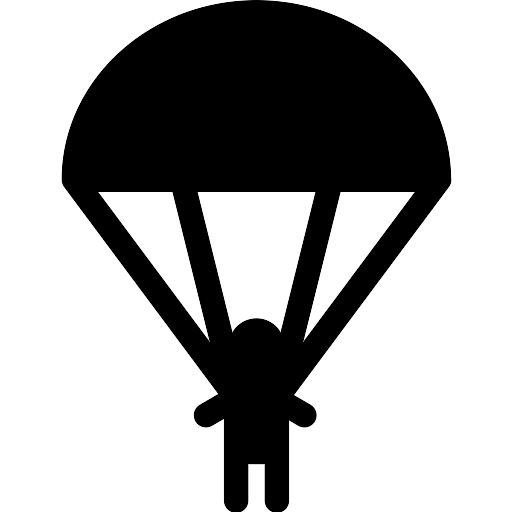
\includegraphics[width=0.3\textwidth]{parachuter.png}
    \end{center}

    ¿Cómo calcularíamos la velocidad de un paracaidista en caída libre justo antes de que abriese el paracaídas? Veamos\dots

\end{frame}

\begin{frame}{El paracaidista: Solución analítica}{Modelación matemática}
    Comencemos con algo simple: ¿Qué hace caer al paracaidista? \pause

    La fuerza de gravedad del paracaidista lo hará caer, y una fuerza opuesta (de resistencia al aire, por ejemplo) \textit{intentará frenarlo} (como soltar una hoja de papel en el aire). \pause
    
    Significa entonces que

    $$\sum_{F_y} = F_g - F_r$$

    donde $F_y$ es la fuerza ejercida sobre el paracaidista, por la fuerza de gravedad $F_g$ y la fuerza de resistencia $F_r$.

\end{frame}

\begin{frame}{El paracaidista: Solución analítica}{Modelación matemática}

    \begin{align*}
        F_g - F_r & = F_y \tag{reescribimos} \\
        F_g - F_r & = ma \tag{por $F=ma$} \\
        mg - F_r & = ma \tag{ditto} \\
        mg - cv & = ma \tag{coeficiente de resistencia por velocidad} \\
        ma & = mg - cv \tag{reescribimos} \\
        m\dv{v}{t} & = mg - cv \tag{$a$ como $\dv{v}{t}$}
    \end{align*}

\end{frame}

\begin{frame}{El paracaidista: Solución analítica}{Modelación matemática}

    \begin{align*}
        m\dv{v}{t} & = mg - cv \tag{de slide anterior} \\
        m\dv{v(t)}{t} & = mg - cv(t) \tag{$v$ como función del tiempo} \\
        \dv{v(t)}{t} + \frac{c}{m}v(t) & = g \tag{despejando $g$}
    \end{align*} \pause

    La ecuación final es una \textbf{ecuación diferencial lineal} de primer orden, la cual tiene una solución \textbf{ya dada}\footnote{P. Dawkins, \url{http://tutorial.math.lamar.edu/Classes/DE/Linear.aspx}} por:

    $$v(t) = e^{-\int p(t)dt} \left( \int q(t) e^{\int p(t)dt} \, dt + k\right)$$

\end{frame}

\begin{frame}{El paracaidista: Solución analítica}{Modelación matemática}

    Y dado a que queremos la velocidad $v(0) = 0$, entonces después de \textit{un poco} de álgebra, llegamos a la solución final

    \begin{equation}
        v(t) = \frac{gm}{c} \left(1 - e^{-\frac{c}{m}t}\right)
    \end{equation}

\end{frame}

\begin{frame}{El paracaidista: Solución analítica}{Modelación matemática}
    Resolvamos ahora para un paracaidista específico de $m = 68.1$kg y con un coeficiente de arrastre $c=12.5$kg/s:

    \bigskip

    $$v(t) = \frac{9.81(68.1)}{12.5} \left(1 - e^{\frac{-12.5}{68.1}t}\right) = 53.44(1 - e^{-0.18355t})$$

    \bigskip

    de la cual podemos obtener una tabla para darnos una idea\dots
    % Please add the following required packages to your document preamble:
% \usepackage{booktabs}
\end{frame}

\begin{frame}{El paracaidista: Solución analítica}{Modelación matemática}

    $$v(t) = 53.44(1 - e^{-0.18355t})$$

    \bigskip
    
    \begin{table}[H]
        \begin{tabular}{@{}lr@{}}
        \toprule
        \textbf{t (s)} & \textbf{v (m/s)} \\ \midrule
        0              & 0.00             \\
        2              & 16.42            \\
        4              & 27.8             \\
        6              & 35.68            \\
        8              & 41.14            \\
        10             & 44.92            \\
        12             & 47.54            \\
        $\infty$       & 53.44            \\ \bottomrule
        \end{tabular}
        \end{table}
\end{frame}

\begin{frame}{El paracaidista: Solución analítica}{Modelación matemática}

    Esta solución se conoce como \alert{solución analítica} o \textbf{exacta} del modelo, ya que podemos obtener \textit{fácilmente} las ecuaciones diferenciales para ello. No siempre es posible hacerlo.

    \bigskip

    Sin embargo, cuando no es posible hallar algo exacto, siempre podemos \textbf{aproximarlo}\dots

\end{frame}

\begin{frame}{El paracaidista: Solución numérica}{Modelación matemática}
    Podemos aproximar la derivada de la velocidad con respecto al tiempo como un \textit{cambio de la velocidad} entre un \textit{cambio en el tiempo}

    \bigskip

    $$\dv{v}{t} \approxeq \frac{\Delta v}{\Delta t} = \frac{v(t_{i+1}) - v(t_i)}{t_{i+1} - t_i}$$

    \bigskip

    Y con ello, podemos reformular nuestro problema

    $$\sum_{F_y} = F_g - F_r$$
\end{frame}

\begin{frame}{El paracaidista: Solución numérica}{Modelación matemática}

    \begin{align*}
        \sum_{F_y} & = F_g - F_r \tag{ecuación original} \\
        ma  & = mg - cv(t_i) \tag{sustituyendo con $F=ma$} \\
        m\dv{v}{t} & = mg - cv(t_i) \tag{$a$ como $\dv{v}{t}$} \\
        m\frac{v(t_{i+1}) - v(t_i)}{t_{i+1} - t_i} & = mg - cv(t_i) \tag{reemplazamos por aproximación}
    \end{align*}

    y despejamos la $v(t_{i+1})$ que es lo que nos interesa\dots 

\end{frame}

\begin{frame}{El paracaidista: Solución numérica}{Modelación matemática}

    $$v(t_{i+1}) = v(t_i) + \left[ g - \frac{c}{m} v(t_i)\right](t_{i+1} - t_i)$$

    Que es una ecuación para determinar la velocidad $v$ para el punto $t_{i+1}$ en el tiempo, usando la pendiente y los valores anteriores de $v$ y $t$. \pause

    $$x_{i+1} = x_i + m \cdot s$$

    \bigskip

    Donde $x_i$ es el valor de la variable independiente en la $i$-ésima iteración, $m$ es la pendiente (o cómo cambia el sistema) y $s$ es el paso (o \textit{step}) de la aproximación.

\end{frame}

\begin{frame}{El paracaidista: Solución numérica}{Modelación matemática}
    \begin{center}
        \Large
        Esta aproximación de forma
        $$x_{i+1} = x_i + m \cdot s$$
        se conoce como \alert{método de Euler}
    \end{center} \pause

    \begin{center}
        \textit{Live coding: Euler's method}
    \end{center}
\end{frame}

\section{Errores}

\begin{frame}{Datos y errores}{Introducción a los métodos numéricos}
    Sin embargo, sigue siendo una aproximación, por lo que existe cierto \alert{error} que vamos a ir cargando poco a poco por el redondeo. \pause

    \bigskip

    El \alert{error real} se calcula como
    $$\varepsilon = \frac{x_{approx}}{x_{real}}$$ \pause

    Si no sabemos el valor real $x_{real}$(muchas veces no lo sabremos) entonces se puede aproximar\dots \pause
    $$\varepsilon_a = \frac{err_{approx}}{val_{approx}}$$ \pause

    Y podemos aproximarlo por cada paso en la simulación

    $$\varepsilon_a = \frac{x_i - x_{i-1}}{x_i}$$

\end{frame}

\begin{frame}{Datos y errores}{Introducción a los métodos numéricos}

    Si siempre vamos a tener errores, ¿cuándo nos detenemos? \pause

    Cuando estemos \textit{lo suficientemente cerca} a lo que determinemos como \textbf{adecuado} para la situación:

    $$\mid \varepsilon_a \mid < \varepsilon_s$$

    donde $\varepsilon_s$ es el \alert{error establecido}. \pause

    Una buena idea es usar un error establecido de
    
    $$\varepsilon_s = 0.5 \times 10^{2-n}$$

    donde el valor será correcto en al menos $n$ \textbf{cifras significativas}.
    
\end{frame}

% What is control flow
% why is it important
% does it exist in math?
% how to represent it
% how to represent it in matlab
% practical cases

% \section*{Referencias}

% \begin{frame}[t]{Referencias}
    % \nocite{bibID01}
    % \nocite{bibID02}

    % \bibliographystyle{IEEE}
    % \bibliography{biblio}
% \end{frame}

\end{document}